\documentclass[tikz,border=5pt]{standalone}
\usepackage{amsmath,amssymb}
\usetikzlibrary{shapes.geometric, arrows.meta, positioning, calc, backgrounds, fit}

\begin{document}
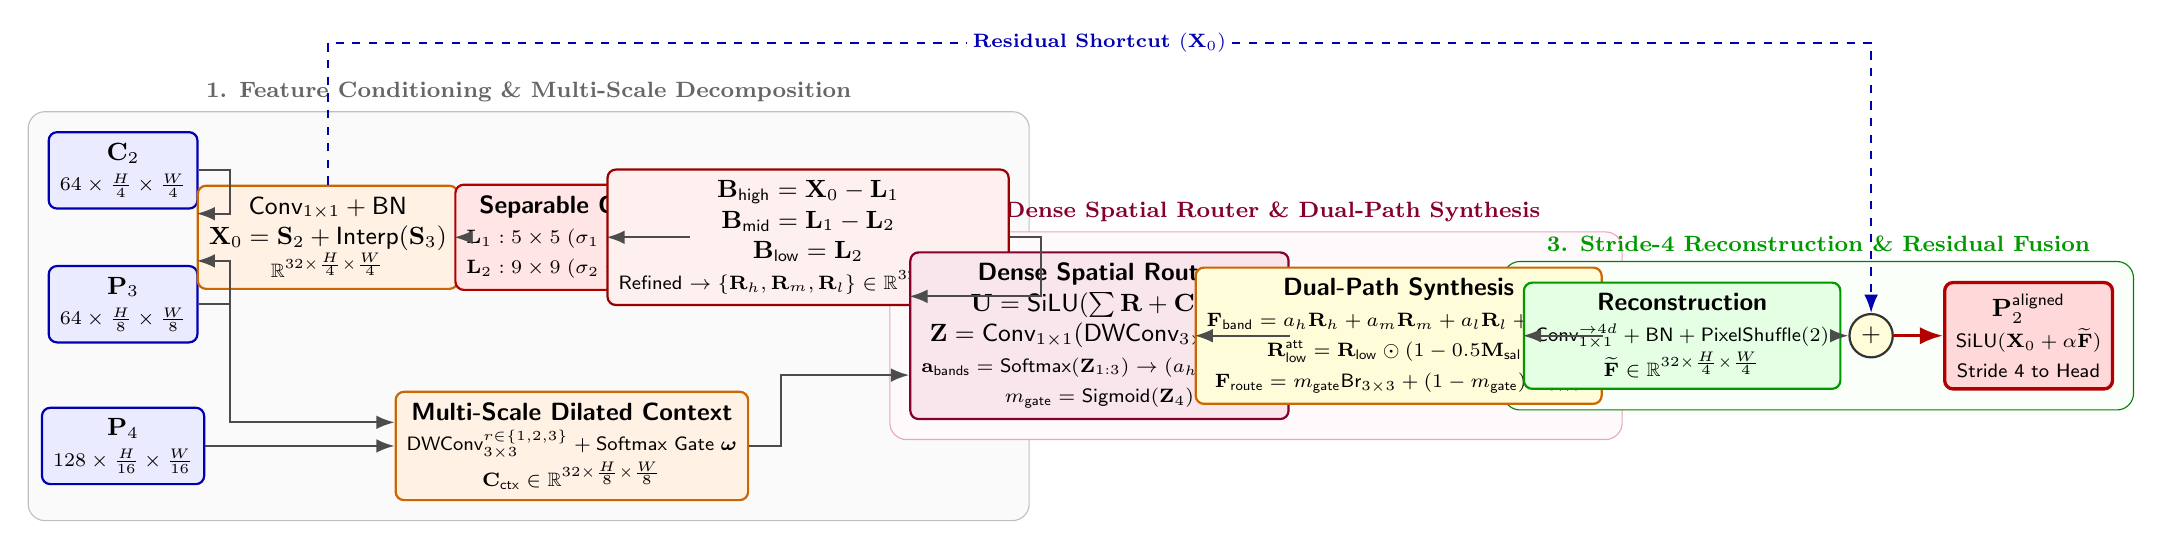
\begin{tikzpicture}[
    >=Latex,
    font=\sffamily\small,
    every node/.style={align=center},
    tensor/.style={rectangle, draw=blue!70!black, fill=blue!8, rounded corners=3pt, thick, minimum height=0.65cm, inner sep=4pt},
    op/.style={rectangle, draw=orange!80!black, fill=orange!10, rounded corners=3pt, thick, minimum height=0.65cm, inner sep=4pt},
    gate/.style={circle, draw=black!80, fill=yellow!15, thick, inner sep=1pt, minimum size=0.55cm},
    arr/.style={->, thick, draw=black!70}
  ]

  % -------------------------------------------------------------
  % Stage 1: Multi-scale Inputs & Scale-Space Decomposition
  % -------------------------------------------------------------
  \node[tensor] (c2) at (0, 2.5) {$\mathbf{C}_2$\\\scriptsize $64\times \frac{H}{4} \times \frac{W}{4}$};
  \node[tensor] (p3) at (0, 0.8) {$\mathbf{P}_3$\\\scriptsize $64\times \frac{H}{8} \times \frac{W}{8}$};
  \node[tensor] (p4) at (0, -1.0) {$\mathbf{P}_4$\\\scriptsize $128\times \frac{H}{16} \times \frac{W}{16}$};

  % Projections and initial fusion X0
  \node[op] (fuse_x0) at (2.6, 1.65) {
    $\text{Conv}_{1\times 1} + \text{BN}$\\
    $\mathbf{X}_0 = \mathbf{S}_2 + \text{Interp}(\mathbf{S}_3)$\\
    \scriptsize $\mathbb{R}^{32 \times \frac{H}{4} \times \frac{W}{4}}$
  };
  \draw[arr] (c2.east) -- ++(0.4,0) |- ($(fuse_x0.west)+(0, 0.3)$);
  \draw[arr] (p3.east) -- ++(0.4,0) |- ($(fuse_x0.west)+(0, -0.3)$);

  % Gaussian Filtering on X0
  \node[op, fill=red!10, draw=red!70!black] (gauss_op) at (5.7, 1.65) {
    \textbf{Separable Gauss}\\
    \scriptsize $\mathbf{L}_1: 5\times 5 \; (\sigma_1 \approx 0.65)$\\
    \scriptsize $\mathbf{L}_2: 9\times 9 \; (\sigma_2 \approx 1.45)$
  };
  \draw[arr] (fuse_x0) -- (gauss_op);

  % Bands
  \node[tensor, fill=red!6, draw=red!60!black] (bands) at (8.7, 1.65) {
    $\mathbf{B}_{\text{high}} = \mathbf{X}_0 - \mathbf{L}_1$\\
    $\mathbf{B}_{\text{mid}} = \mathbf{L}_1 - \mathbf{L}_2$\\
    $\mathbf{B}_{\text{low}} = \mathbf{L}_2$\\
    \scriptsize Refined $\to \{\mathbf{R}_h, \mathbf{R}_m, \mathbf{R}_l\} \in \mathbb{R}^{32 \times \frac{H}{8} \times \frac{W}{8}}$
  };
  \draw[arr] (gauss_op) -- (bands);

  % Context branch C_ctx
  \node[op] (ctx_mod) at (5.7, -1.0) {
    \textbf{Multi-Scale Dilated Context}\\
    \scriptsize $\text{DWConv}_{3\times 3}^{r \in \{1,2,3\}} + \text{Softmax Gate} \;\boldsymbol{\omega}$\\
    \scriptsize $\mathbf{C}_{\text{ctx}} \in \mathbb{R}^{32 \times \frac{H}{8} \times \frac{W}{8}}$
  };
  \draw[arr] (p4) -- (ctx_mod);
  \draw[arr] (p3.east) -- ++(0.4,0) |- ($(ctx_mod.west)+(0, 0.3)$);

  % -------------------------------------------------------------
  % Stage 2: Spatial Router (Dense DWConv + 1x1)
  % -------------------------------------------------------------
  \node[op, fill=purple!10, draw=purple!70!black] (spatial_router) at (12.4, 0.4) {
    \textbf{Dense Spatial Router}\\
    $\mathbf{U} = \text{SiLU}(\sum \mathbf{R} + \mathbf{C}_{\text{ctx}})$\\
    $\mathbf{Z} = \text{Conv}_{1\times 1}(\text{DWConv}_{3\times 3}(\mathbf{U}))$\\
    \scriptsize $\mathbf{a}_{\text{bands}} = \text{Softmax}(\mathbf{Z}_{1:3}) \to (a_h, a_m, a_l)$\\
    \scriptsize $m_{\text{gate}} = \text{Sigmoid}(\mathbf{Z}_4)$
  };
  \draw[arr] (bands.east) -- ++(0.4,0) |- ($(spatial_router.west)+(0, 0.5)$);
  \draw[arr] (ctx_mod.east) -- ++(0.4,0) |- ($(spatial_router.west)+(0, -0.5)$);

  % Synthesis node
  \node[op, fill=yellow!15, draw=orange!80!black] (synth) at (16.2, 0.4) {
    \textbf{Dual-Path Synthesis}\\
    \scriptsize $\mathbf{F}_{\text{band}} = a_h \mathbf{R}_h + a_m \mathbf{R}_m + a_l \mathbf{R}_l + \gamma_h \mathbf{R}_h$\\
    \scriptsize $\mathbf{R}_{\text{low}}^{\text{att}} = \mathbf{R}_{\text{low}} \odot (1 - 0.5\mathbf{M}_{\text{sal}})$\\
    \scriptsize $\mathbf{F}_{\text{route}} = m_{\text{gate}} \text{Br}_{3\times 3} + (1 - m_{\text{gate}}) \text{Br}_{5\times 5}$
  };
  \draw[arr] (spatial_router) -- (synth);

  % -------------------------------------------------------------
  % Stage 3: Stride-4 Reconstruction & Aligned Residual Addition
  % -------------------------------------------------------------
  \node[op, fill=green!10, draw=green!60!black] (recon) at (19.8, 0.4) {
    \textbf{Reconstruction}\\
    \scriptsize $\text{Conv}_{1\times 1}^{\to 4d} + \text{BN} + \text{PixelShuffle}(2)$\\
    \scriptsize $\widetilde{\mathbf{F}} \in \mathbb{R}^{32 \times \frac{H}{4} \times \frac{W}{4}}$
  };
  \draw[arr] (synth) -- (recon);

  \node[gate] (add) at (22.2, 0.4) {$+$};
  \draw[arr] (recon) -- (add);

  % Residual shortcut from X0
  \draw[arr, dashed, blue!70!black] (fuse_x0.north) -- ++(0, 1.8) -| node[pos=0.25, fill=white, inner sep=2pt, font=\scriptsize\bfseries] {Residual Shortcut $(\mathbf{X}_0)$} (add.north);

  % Output P2 aligned
  \node[tensor, fill=red!15, draw=red!70!black, very thick] (p2_out) at (24.2, 0.4) {
    $\mathbf{P}_2^{\text{aligned}}$\\
    \scriptsize $\text{SiLU}(\mathbf{X}_0 + \alpha \widetilde{\mathbf{F}})$\\
    \scriptsize Stride 4 to Head
  };
  \draw[arr, very thick, red!70!black] (add) -- (p2_out);

  % Section Group Boxes
  \begin{scope}[on background layer]
    \node[draw=black!25, fill=black!2, rounded corners=6pt, fit=(c2)(fuse_x0)(gauss_op)(bands)(ctx_mod), inner sep=7pt, label={[font=\footnotesize\bfseries, text=black!60]above:1. Feature Conditioning \& Multi-Scale Decomposition}] {};
    \node[draw=purple!35, fill=purple!2, rounded corners=6pt, fit=(spatial_router)(synth), inner sep=7pt, label={[font=\footnotesize\bfseries, text=purple!70!black]above:2. Dense Spatial Router \& Dual-Path Synthesis}] {};
    \node[draw=green!50!black, fill=green!2, rounded corners=6pt, fit=(recon)(add)(p2_out), inner sep=7pt, label={[font=\footnotesize\bfseries, text=green!60!black]above:3. Stride-4 Reconstruction \& Residual Fusion}] {};
  \end{scope}

\end{tikzpicture}
\end{document}
